\documentclass[a4paper,11pt]{article}
\usepackage[utf8]{inputenc}
\usepackage[english]{babel}
\usepackage[colorlinks=true, urlcolor=black, linkcolor=black]{hyperref}
\usepackage[margin=3cm]{geometry}
\usepackage{parskip}
\usepackage{hyperref}
\usepackage{graphicx}
\usepackage{xcolor}
\usepackage{fancyvrb}

\setlength{\parindent}{3em}

\author{
	\Large Cerezo Pomykol, Jan\\ \href{mailto:j.cerezo@alumnos.upm.es}{\small\texttt{j.cerezo@alumnos.upm.es}}
}

\title{\textbf{\Huge Practical Application 2} \\
		\Large Machine Learning}

\date{\Large November 22, 2022}

\begin{document}
\maketitle
\vfill

\tableofcontents
\newpage

\section{Introduction}
\label{sec:introduction}

The goal of this practical application is to study how feature subset selection (FSS) affects different machine learning models. Specifically how they perform with a dataset with all variables and datasets obtained from a univariate filter, a multivariate filter, and a multivariate wrapper. The selected classification models and \textit{meta-classifiers} are the following:

\begin{itemize}
\item Logistic Regression.
\item Naive Bayes.
\item Tree Augmented Naive Bayes.
\item Linear Discriminant Analysis.
\item Fusion.
\item Stacking.
\item Bagging.
\item Random Forest.
\item Boosting.
\item Naive Bayes Tree.
\item Logistic Model Trees.
\end{itemize}

For this assignment, the dataset chosen \cite{misc_dry_bean_dataset_602}\cite{KOKLU2020105507} contains data about instances of dry beans, which was created from images of 13,611 grains of 7 different varieties.

The rest of the document has the following structure. Firstly, de dataset is analysed in the \hyperref[sec:problem]{Problem Description}, later the methodology is specified in the \hyperref[sec:methodology]{Methodology section}. Subsequently the results are shown in the \hyperref[sec:results]{Results section}, and finally they are analysed in the \hyperref[sec:discussion]{Discussion} and \hyperref[sec:conclusion]{Conclusion} sections.

\section{Problem Description}
\label{sec:problem}

The dataset contains 13,611 instances created from images of dry beans of 7 different varieties. There are a total of 17 attributes (16 plus the class column) and their significance is the following:

\begin{itemize}
\setlength\itemsep{-1ex}
\item[1] \textbf{Area} (A): The area of a bean zone and the number of pixels within its boundaries.
\item[2] \textbf{Perimeter} (P): Length of its border.
\item[3] \textbf{Major axis length} (L): Length of the longest line that can be drawn from a bean.
\item[4] \textbf{Minor axis length} (l): Length of the longest line that can be drawn from the bean while standing perpendicular to the main axis.
\item[5] \textbf{Aspect ratio} (K): Relationship between L and l.
\item[6] \textbf{Eccentricity} (Ec): Eccentricity of the ellipse having the same moments as the region.
\item[7] \textbf{Convex area} (C): Number of pixels in the smallest convex polygon that can contain the area of a bean seed.
\item[8] \textbf{Equivalent diameter} (Ed): The diameter of a circle having the same area as a bean seed area.
\item[9] \textbf{Extent} (Ex): The ratio of the pixels in the bounding box to the bean area.
\item[10] \textbf{Solidity} (S): Also known as convexity. The ratio of the pixels in the convex shell to those found in beans.
\item[11] \textbf{Roundness} (R): Calculated with the following formula: $\frac{4\pi A}{P^2}$
\item[12] \textbf{Compactness} (CO): Measures the roundness of an object: $\frac{Ed}{L}$
\item[13] \textbf{ShapeFactor1} (SF1)
\item[14] \textbf{ShapeFactor2} (SF2)
\item[15] \textbf{ShapeFactor3} (SF3)
\item[16] \textbf{ShapeFactor4} (SF4)
\item[17] \textbf{Class}: Seker, Barbunya, Bombay, Cali, Dermosan, Horoz and Sira.
\end{itemize}

All attributes are numeric, except the class which is nominal. Additionally, there are no \textit{meta-attributes} such as instance or object identifiers, so there is no need to remove any column. \autoref{tab:table1} shows more information about the ranges of values and \autoref{tab:table2} shows the number of instances of each class.

\begin{table}[h]
\centering
\begin{tabular}{||l|l|l|l||}
	\hline
	No. & Name & Min. & Max.\\
	\hline
	1 & Area & 20420 & 254616\\
	2 & Perimeter & 524.736 & 1985.37\\
	3 & Major axis length & 183.601 & 738.86\\
	4 & Minor axis length & 122.513 & 460.198\\
	5 & Aspect ratio & 1.025 & 2.43\\
	6 & Eccentricity & 0.219 & 0.911\\
	7 & Convex area & 20684 & 263261\\
	8 & Equivalent diameter & 161.244 & 569.374\\
	9 & Extent & 0.555 & 0.866\\
	10 & Solidity & 0.919 & 0.995\\
	11 & Roundness & 0.49 & 0.991\\
	12 & Compactness & 0.641 & 0.987\\
	13 & ShapeFactor1 & 0.003 & 0.01\\
	14 & ShapeFactor2 & 0.001 & 0.004\\
	15 & ShapeFactor3 & 0.41 & 0.975\\
	16 & ShapeFactor4 & 0.948 & 1\\
	17 & Class & - & -\\
	\hline
\end{tabular}
\caption{Value ranges of each variable.}
\label{tab:table1}
\end{table}

\begin{table}[h]
\centering
\begin{tabular}{||l|l||}
	\hline
	Class & n\\
	\hline
	SEKER & 2027\\
	BARBUNYA & 1322\\
	BOMBAY & 522\\
	CALI & 1630\\
	HOROZ & 1928\\
	SIRA & 2636\\
	DERMASON & 3546\\
	\hline
\end{tabular}
\caption{Number of instances per class.}
\label{tab:table2}
\end{table}

Since there are some variables with high values compared to others (for example Area compared to Extent); normalization is necessary.

\section{Methodology}
\label{sec:methodology}

\subsection{Software}
\label{subsec:software}

For this practical application, Weka \cite{weka} has been used to perform the training and evaluation of all models, as well as the normalization of the dataset. Besides from normalization of the dataset, there is no need to perform more pre-processing. There are no missing values and all variables are numerical (except the class).

\subsection{Evaluation}
\label{subsec:evaluation}

The evaluation of each model will be conducted with cross validation with 10 folds. Because each class has different weight (different number of instances) the confusion matrix will be discussed as well in some cases. Besides the accuracy, training time will also be considered.

\subsection{Classification Algorithms}
\label{subsec:algorithms}

The following machine learning algorithms have been evaluated.

\begin{itemize}
\item \textbf{Logistic Regression}. Default parameters.
\item \textbf{Naive Bayes}. Default parameters.
\item \textbf{Tree Augmented Naive Bayes}. With TAN search algorithm.
\item \textbf{Linear Discriminant Analysis}. Default parameters.
\item \textbf{Fusion}. With the following classifiers: Naive Bayes, TAN and LDA. The combination rule used is the Average.
\item \textbf{Stacking}. The \textit{meta-classifier} is set to Naive Bayes. The classifiers are TAN and LDA.
\item \textbf{Bagging}. With Naive Bayes classifier.
\item \textbf{Random Forest}. Default parameters.
\item \textbf{Boosting}. With Naive Bayes classifier.
\item \textbf{Naive Bayes Tree}. Default parameters.
\item \textbf{Logistic Model Trees}. Default parameters.
\end{itemize}

\autoref{tab:table3} shows the Weka function associated to each algorithm.

\begin{table}[h]
\centering
\begin{tabular}{||l|l||}
	\hline
	Algorithm & Weka Function\\
	\hline
	Logistic Regression & functions.Logistic\\
	Naive Bayes & bayes.NaiveBayes\\
	Tree Augmented Naive Bayes & bayes.BayesNet\\
	Linear Discriminant Analysis & functions.LDA\\
	Fusion & meta.Vote \\
	Stacking & meta.Stacking\\
	Bagging & meta.Bagging\\
	Random Forest & trees.RandomForest\\
	Boosting & meta.AdaBoostM1\\
	Naive Bayes Tree & trees.NBTree\\
	Logistic Model Trees & trees.LMT\\
	\hline
\end{tabular}
\caption{Weka implementation of each algorithm.}
\label{tab:table3}
\end{table}

\subsection{Feature Subset Selection}
\label{subsec:fss}

The selection of features has been performed with the following algorithms. \autoref{tab:table4} shows the Weka function associated to each method.

\begin{itemize}
\setlength\itemsep{-1ex}
\item \textbf{No FSS}. The original dataset was used.
\item \textbf{Univariant Filter}. Evaluates the worth of each attribute by measuring the information gain with respect to the class. The threshold used for this dataset is 1.2.
\item \textbf{Multivariant Filter}. Evaluates the worth of a subset of attributes by considering the individual predictive ability of each feature along with the degree of redundancy between them.
\item \textbf{Wrapper Approach}. Evaluates each subset of attributes with the estimated performance of a classifier built with this subset of attributes.
\end{itemize}

\begin{table}[h]
\centering
\begin{tabular}{||l|l||}
	\hline
	FSS algorithm & Weka Function\\
	\hline
	No FSS & -\\
	Univariant Filter & attributeSelection.InfoGainAttributeEval\\
	Multivariant Filter & attributeSelection.CfsSubsetEval\\
	Wrapper Approach & attributeSelection.WrapperSubsetEval\\
	\hline
\end{tabular}
\caption{Weka implementation of each FSS algorithm.}
\label{tab:table4}
\end{table}

Note that the optimization of each classification model and feature selection method is not part of this practical application.

\section{Results}
\label{sec:results}

This section includes the scores obtained with each classifier (\hyperref[subsec:algorithms]{section 3.3}) and each Feature Subset Selection approach (\hyperref[subsec:fss]{section 3.4}). \autoref{tab:table5} shows the attributes selected by each method.

\begin{table}[h]
\centering
\begin{tabular}{||l|c|c|c|c|c|c|c|c|c|c|c|c|c|c||}
	\hline
	Attribute &
	\rotatebox[origin=c]{90}{No FSS} &
	\rotatebox[origin=c]{90}{Univariant} &
	\rotatebox[origin=c]{90}{Multivariant} &
	\rotatebox[origin=c]{90}{Wrapper (Logistic)} &
	\rotatebox[origin=c]{90}{Wrapper (Naive Bayes)} &
	\rotatebox[origin=c]{90}{Wrapper (TAN)} &
	\rotatebox[origin=c]{90}{Wrapper (LDA)} &
	\rotatebox[origin=c]{90}{Wrapper (Fusion)} &
	\rotatebox[origin=c]{90}{Wrapper (Stacking)} &
	\rotatebox[origin=c]{90}{Wrapper (Bagging)} &
	\rotatebox[origin=c]{90}{Wrapper (Random Forest)} &
	\rotatebox[origin=c]{90}{Wrapper (Boosting)} &
	\rotatebox[origin=c]{90}{Wrapper (NBTree)} &
	\rotatebox[origin=c]{90}{Wrapper (LMT)}\\
	\hline
	Area &  & $\bullet$ & & & & & $\bullet$ & & & $\bullet$ & $\bullet$ & $\bullet$ & & $\bullet$\\
    Perimeter & $\bullet$ & $\bullet$ & $\bullet$ & $\bullet$ & $\bullet$ & $\bullet$ & $\bullet$ & $\bullet$ & $\bullet$ & $\bullet$ & & $\bullet$ & $\bullet$ & $\bullet$\\
    MajorAxisLength & $\bullet$ & $\bullet$ & $\bullet$ & $\bullet$ & & & & & $\bullet$ & & $\bullet$ & & & $\bullet$\\
    MinorAxisLength & $\bullet$ & $\bullet$ & $\bullet$ & $\bullet$ & & $\bullet$ & & $\bullet$ & & & & & $\bullet$ & \\
    AspectRatio & $\bullet$ & & $\bullet$ & & & $\bullet$ & & & $\bullet$ & & & & & \\
    Eccentricity & $\bullet$ & & & & & & & & $\bullet$ & & & & & \\
    ConvexArea & $\bullet$ & $\bullet$ & $\bullet$ & $\bullet$ & & & $\bullet$ & & $\bullet$ & & & & & $\bullet$\\
    EquivDiameter & $\bullet$ & $\bullet$ & & $\bullet$ & & & & & $\bullet$ & & & & & $\bullet$\\
    Extent & $\bullet$ & & $\bullet$ & $\bullet$ & & $\bullet$ & $\bullet$ & $\bullet$ & $\bullet$ & $\bullet$ & $\bullet$ & $\bullet$ & & \\
    Solidity & $\bullet$ & & & $\bullet$ & & & & $\bullet$ & & $\bullet$ & $\bullet$ & & $\bullet$ & $\bullet$\\
    Roundness & $\bullet$ & & $\bullet$ & $\bullet$ & $\bullet$ & $\bullet$ & & $\bullet$ & $\bullet$ & $\bullet$ & $\bullet$ & & $\bullet$ & $\bullet$\\
    Compactness & $\bullet$ & & $\bullet$ & & $\bullet$ & $\bullet$ & $\bullet$ & $\bullet$ & & $\bullet$ & $\bullet$ & & $\bullet$ & \\
    ShapeFactor1 & $\bullet$ & $\bullet$ & $\bullet$ & $\bullet$ & $\bullet$ & $\bullet$ & & & & $\bullet$ & $\bullet$ & & & \\
    ShapeFactor2 & $\bullet$ & $\bullet$ & $\bullet$ & $\bullet$ & & & & & $\bullet$ & $\bullet$ & & & & $\bullet$\\
    ShapeFactor3 & $\bullet$ & & & & & & & & & & $\bullet$ & $\bullet$ & & \\
	ShapeFactor4 & $\bullet$ & & $\bullet$ & $\bullet$ & $\bullet$ & $\bullet$ & $\bullet$ & $\bullet$ & $\bullet$ & $\bullet$ & $\bullet$ & & $\bullet$ & $\bullet$\\
    \hline
    \textbf{N attributes} & 16 & 8 & 11 & 11 & 5 & 8 & 6 & 7 & 10 & 9 & 9 & 4 & 6 & 9\\
    \hline
\end{tabular}
\caption{Attributes selected with each FSS algorithm.}
\label{tab:table5}
\end{table}

%Dry_Bean_Dataset_Wrapper_RIPPER.arff

\autoref{tab:table6} shows the score of each classification algorithm with all datasets obtained from each Feature Subset Selection method described, and \autoref{tab:table7} shows the training time of each model. Note that full outputs of every model are not listed due to the limited extension of this assignment. The full version of each result report including the confusion matrices can be found in \cite{repo}.

\begin{table}[h]
\centering
\resizebox{0.95\textwidth}{!}{
\begin{tabular}{||l|l|l|l|l|l|l|l|l|l|l|l||}
	\hline
	Dataset &
	\rotatebox[origin=c]{90}{Logistic} &
	\rotatebox[origin=c]{90}{Naive Bayes} &
	\rotatebox[origin=c]{90}{TAN} &
	\rotatebox[origin=c]{90}{LDA} &
	\rotatebox[origin=c]{90}{Fusion} &
	\rotatebox[origin=c]{90}{Stacking} &
	\rotatebox[origin=c]{90}{Bagging} &
	\rotatebox[origin=c]{90}{Random Forest} &
	\rotatebox[origin=c]{90}{Boosting} &
	\rotatebox[origin=c]{90}{NBTree} &
	\rotatebox[origin=c]{90}{LMT}\\
	\hline
	Original & 92.60 & 89.71 & 91.47 & 90.18 & 91.26 & 91.28 & 89.72 & 92.52 & 89.71 & 89.57 & 92.49\\
	Uni. Filter & 92.14 & 84.09 & 89.90 & 89.22 & 90.00 & 90.29 & 84.03 & 91.04 & 84.09 & 87.67 & 91.94\\
	Mult. Filter & 92.57 & 90.20 & 91.24 & 90.05 & 91.58 & 91.74 & 90.31 & 92.47 & 90.20 & 90.63 & 92.41\\
	Wr. (Logistic) & 92.70 & 89.01 & 91.47 & 90.03 & 91.47 & 91.53 & 89.08 & 92.53 & 89.01 & 89.66 & 89.01\\
	Wr. (N. Bayes) & 92.09 & 91.23 & 91.54 & 89.84 & 89.01 & 91.77 & 91.21 & 92.16 & 91.23 & 91.55 & 92.16\\
	Wr. (TAN) & 92.36 & 90.76 & 91.60 & 89.83 & 91.72 & 91.62 & 90.80 & 92.33 & 90.76 & 90.69 & 92.27\\
	Wr. (LDA) & 92.30 & 88.23 & 90.42 & 91.17 & 91.35 & 91.56 & 88.34 & 91.74 & 88.23 & 89.57 & 92.35\\
	Wr. (Fusion) & 92.39 & 91.05 & 91.29 & 90.58 & 91.91 & 91.24 & 91.05 & 92.68 & 91.05 & 90.88 & 92.44\\
	Wr. (Stacking) & 92.55 & 89.42 & 91.66 & 89.86 & 91.38 & 92.20 & 89.45 & 92.46 & 89.42 & 89.97 & 92.41\\
	Wr. (Bagging) & 92.53 & 90.77 & 91.44 & 89.45 & 91.58 & 91.78 & 90.75 & 92.70 & 90.77 & 90.90 & 92.54\\
	Wr. (R. Forest) & 92.38 & 90.66 & 91.27 & 89.72 & 91.58 & 91.53 & 90.65 & 92.84 & 90.66 & 90.33 & 92.56\\
	Wr. (Boosting) & 91.12 & 80.83 & 89.60 & 88.85 & 89.39 & 89.69 & 80.89 & 91.11 & 80.83 & 89.48 & 91.42\\
	Wr. (NBTree) & 92.21 & 91.22 & 91.24 & 90.56 & 91.89 & 91.17 & 91.22 & 92.46 & 91.22 & 91.27 & 92.27\\
	Wr. (LMT) & 92.45 & 84.75 & 91.02 & 90.32 & 91.22 & 91.30 & 84.80 & 92.28 & 84.75 & 89.82 & 92.52\\
    \hline 
\end{tabular}
}
\caption{Scores of all classifiers with all obtained datasets (percentage of correctly classified instances).}
\label{tab:table6}
\end{table}

\begin{table}[h]
\centering
\resizebox{0.95\textwidth}{!}{
\begin{tabular}{||l|l|l|l|l|l|l|l|l|l|l|l||}
	\hline
	Dataset &
	\rotatebox[origin=c]{90}{Logistic} &
	\rotatebox[origin=c]{90}{Naive Bayes} &
	\rotatebox[origin=c]{90}{TAN} &
	\rotatebox[origin=c]{90}{LDA} &
	\rotatebox[origin=c]{90}{Fusion} &
	\rotatebox[origin=c]{90}{Stacking} &
	\rotatebox[origin=c]{90}{Bagging} &
	\rotatebox[origin=c]{90}{Random Forest} &
	\rotatebox[origin=c]{90}{Boosting} &
	\rotatebox[origin=c]{90}{NBTree} &
	\rotatebox[origin=c]{90}{LMT}\\
	\hline 
	Original & 57.5 & 0.02 & 0.14 & 0.02 & 0.17 & 1.67 & 0.19 & 3.99 & 1.17 & 11.51 & 14.38\\
	Uni. Filter & 2.39 & 0.01 & 0.06 & 0.01 & 0.07 & 0.7 & 0.09 & 3.1 & 0.61 & 5.83 & 10.58\\
	Mult. Filter & 3.89 & 0.01 & 0.09 & 0.01 & 0.11 & 1.06 & 0.15 & 3.18 & 0.84 & 7.17 & 11.41\\
	Wr. (Logistic) & 5.81 & 0.01 & 0.09 & 0.01 & 0.11 & 1.06 & 0.13 & 3.21 & 1.14 & 10.54 & 12.27\\
	Wr. (N. Bayes) & 1.37 & 0.01 & 0.03 & 0.01 & 0.04 & 0.45 & 0.08 & 2.38 & 0.46 & 1.92 & 8.39\\
	Wr. (TAN) & 2.18 & 0.01 & 0.06 & 0.01 & 0.07 & 0.74 & 0.1 & 3.14 & 0.51 & 6.52 & 9.58\\
	Wr. (LDA) & 1.99 & 0.01 & 0.04 & 0.01 & 0.07 & 0.53 & 0.08 & 2.48 & 0.39 & 2.9 & 13\\
	Wr. (Fusion) & 1.97 & 0.01 & 0.05 & 0.01 & 0.06 & 0.63 & 0.09 & 2.46 & 0.58 & 5.23 & 9.86\\
	Wr. (Stacking) & 2.69 & 0.01 & 0.07 & 0.01 & 0.09 & 0.92 & 0.12 & 3.21 & 0.99 & 8.71 & 10.74\\
	Wr. (Bagging) & 2.44 & 0.01 & 0.07 & 0.01 & 0.09 & 0.82 & 0.12 & 3.17 & 0.67 & 5.63 & 10.57\\
	Wr. (R. Forest) & 2.51 & 0.01 & 0.07 & 0.01 & 0.09 & 0.82 & 0.11 & 3.21 & 0.87 & 8.61 & 10.33\\
	Wr. (Boosting) & 0.97 & 0.01 & 0.03 & 0.01 & 0.03 & 0.36 & 0.06 & 2.18 & 0.46 & 1.43 & 8.26\\
	Wr. (NBTree) & 0.96 & 0.01 & 0.04 & 0.01 & 0.06 & 0.53 & 0.09 & 2.44 & 0.45 & 3.96 & 9.05\\
	Wr. (LMT) & 7.95 & 0.01 & 0.06 & 0.01 & 0.08 & 0.83 & 0.11 & 3.28 & 0.56 & 8.26 & 16.41\\
    \hline 
\end{tabular}
}
\caption{Training time in seconds.}
\label{tab:table7}
\end{table}

\section{Discussion}
\label{sec:discussion}

Generally, the models trained obtained a score of at least 90\% in most cases. However, the results do not differ greatly from each other. The greatest precision obtained is 92.84\%, which was achieved with the dataset obtained from the Wrapper Algorithm (Random Forest), and the Random Forest classifier.

Overall, the best performing models are the Logistic Regression, the Random Forest, and the Logistic Model Tree. The worst being the Linear Discriminant Analysis classifier, and the Bagging and Boosting \textit{meta-classifiers}.

Respecting to training time, the fastest models are the Naive Bayes, Tree Augmented Naive Bayes and Linear Discriminant Analysis classifiers, while the slowest are the Logistic Regression and the Logistic Model Trees.

Regarding the selection of features of this dataset, not all variables are needed to obtain models that perform as well as the model generated from all attributes. \autoref{tab:table5} shows that most Feature Subset Selection methods selected the Perimeter, Extent, Roundness and ShapeFactor4, which resembles the importance of these attributes. Similar results were obtained in the previous assignment, where the most selected features were the Perimeter, Roundness, ShapeFactor1 and ShapeFactor4.

In the case of the Logistic Regression classifier, the scores achieved are amongst the highest, the best one obtained with the dataset from the Wrapper with Logistic Regression classifier. This score is better than the one obtained from the original dataset, which suggests that the most relevant features for this classifier are the Perimeter, MajorAxisLength, MinorAxisLength, ConvexArea, EquivDiameter, Extent, Solidity, Roundness, ShapeFactor1, ShapeFactor2 and ShapeFactor4. \autoref{fig:logistic} displays the output of the coefficients and odds ratios for the dataset obtained with the Wrapper approach (with Naive Bayes). As we can see there are some variables that are more explanatory than others. For instance, in the class BARBUNYA the most relevant attribute is the perimeter.

\begin{figure}[h]
\centering
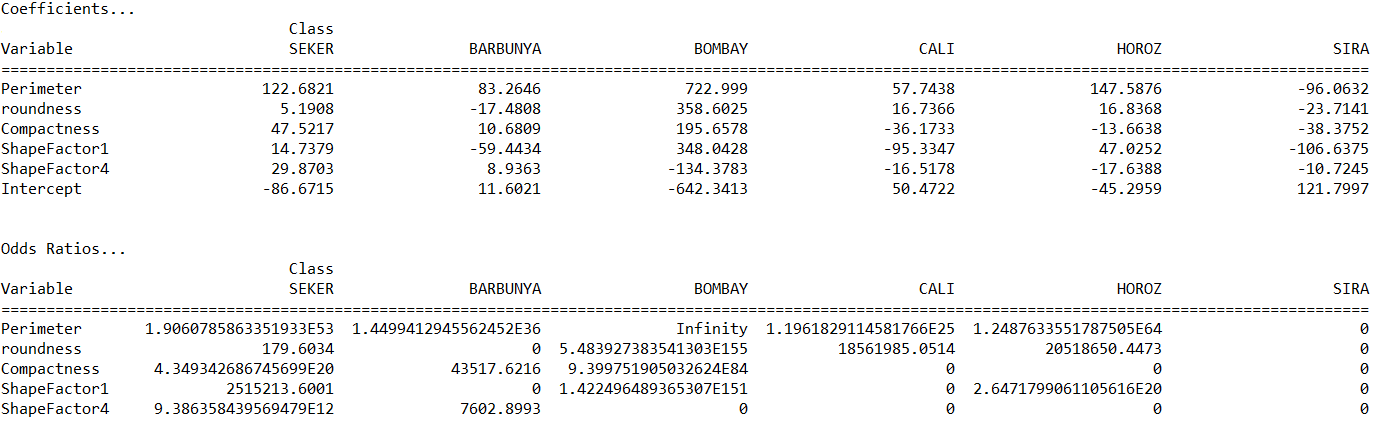
\includegraphics[width=0.95\textwidth]{logistic}
\caption{Coefficients and odds ratios of the Logistic Regression model.}
\label{fig:logistic}
\end{figure}

The Naive Bayes classifier trained the model significantly faster than the others, while reducing slightly the score. \autoref{fig:naivebayes} shows a simplified output of the model obtained with the reduced dataset, and the confusion matrix.

\begin{figure}[h]
\centering
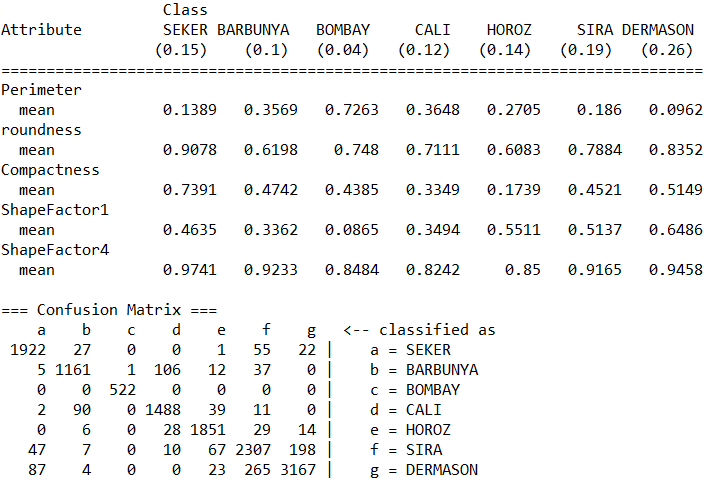
\includegraphics[width=0.8\textwidth]{naivebayes}
\caption{Model and confusion matrix of the Naive Bayes classifier.}
\label{fig:naivebayes}
\end{figure}

In this case, most misclassified instances are from the classes SIRA and DERMASON. This is because both classes have similar mean values in all attributes. From this output we can also deduce what types of beans have higher perimeter (the largest are from the class BOMBAY). Additionally, most classes have high roundness (above 0.7), except BARBUNYA and HOROZ, which suggests that these two varieties have longer shapes. Overall the most discriminant attributes are the Perimeter, Compactness and ShapeFactor1.

The Tree Augmented Naive Bayes classifier obtained better scores than the standard Naive Bayes classifier, while slightly increasing the training times. \autoref{fig:tan} shows the tree obtained from the reduced dataset with the Wrapper approach (Naive Bayes), and tables containing probability distributions of each class for the attributes Class and ShapeFactor1.

\begin{figure}[h]
\centering
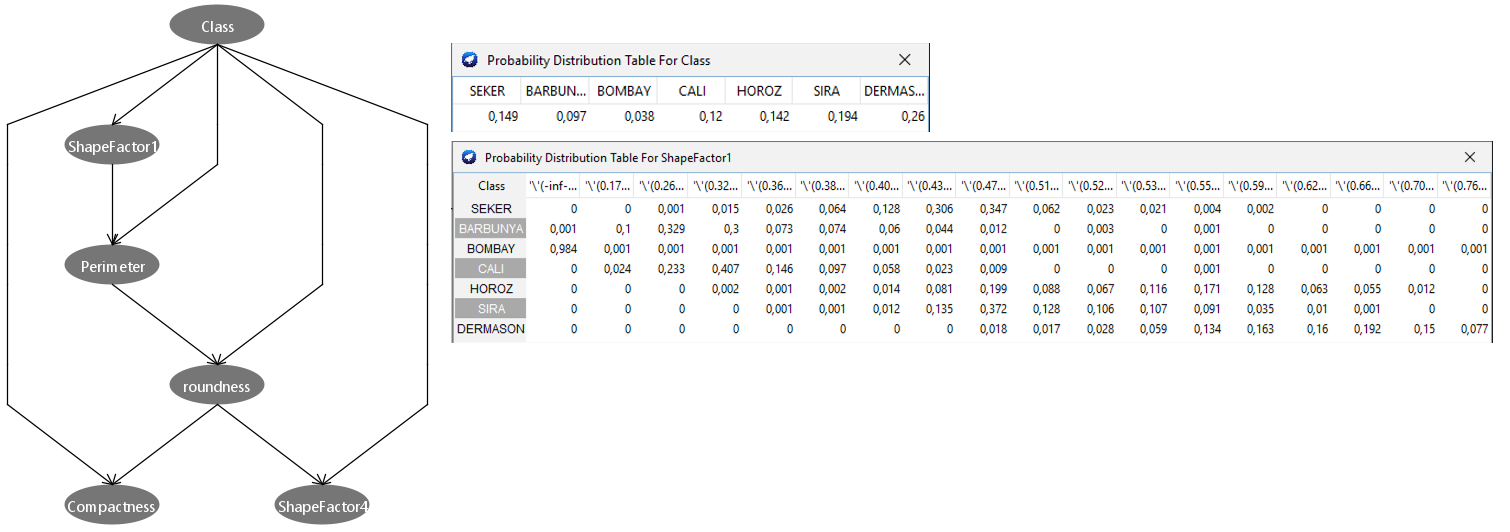
\includegraphics[width=0.95\textwidth]{TAN}
\caption{Tree obtained from the Tree Augmented Naive Bayes classifier.}
\label{fig:tan}
\end{figure}

The Linear Discriminant Analysis obtained better scores than the standard Naive Bayes, while taking the same amount of time to train the models. \autoref{fig:lda} shows the mean vectors of some classes of the model obtained from the original dataset. In this case we can see that the least explanatory attributes are the Extent, Solidity and ShapeFactor4.

\begin{figure}[h]
\centering
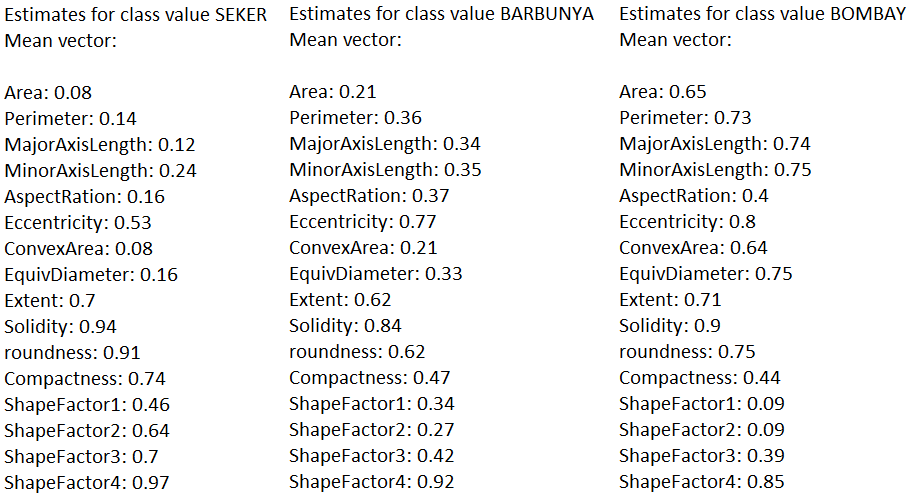
\includegraphics[width=0.8\textwidth]{LDA}
\caption{Mean vectors of classes SEKER, BARBUNYA and BOMBAY (LDA model).}
\label{fig:lda}
\end{figure}

In the case of the meta-classifiers, the scores are diverse. The best performing models are the Fusion, Stacking, Random Forest and Logistic Model Trees. Note that the last two are significantly slower to train.

Inspecting \autoref{tab:table6} we can deduce that in most cases the reduced datasets obtain similar or better scores when compared to the original dataset. This is because there are variables that provide no additional information, in other words, there are dependent or irrelevant variables in the dataset. As stated in the \hyperref[sec:problem]{Problem Description section}, there are some variables that are calculated from others. For instance, the \textit{Roundness} is obtained from the \textit{Area} and the \textit{Perimeter}, and the \textit{Compactness} from the \textit{Equivalent diameter} and the \textit{Major axis length}. Additionally, there are some attributes that are fundamentally related, such as the \textit{Area} and the \textit{Perimeter}.

Overall, all the reduced datasets obtained similar scores compared to the original dataset. The cause of this is the redundancy of some variables. However, the scores are not close to 100\%, probably because the dataset contains multiple irrelevant attributes, and the isolated \textit{important} features need more complex models to fit the distribution. This conclusion is also achieved in the previous assignment.

\section{Conclusion}
\label{sec:conclusion}

In this practical application, a dataset of dry beans with 13,611 instances and 17 features (Including the class) was analysed with different attribute selection methods and different classifiers with a 10-fold cross-validation test approach. The dataset contains instances of seven different classes. The only pre-processing needed was the normalization of the dataset, since there are no missing values or nominal variables (except the class column).

Different datasets were obtained from the original by extracting features with a Univariate Filter, Multivariate Filter, and different Wrapper approaches. All of which were tested with the following classifiers: Logistic Regression, Naive Bayes, Tree Augmented Naive Bayes and Linear Discriminant Analysis. Additionally, the following \textit{meta-classifiers} were used as well: Fusion, Stacking, Bagging, Random Forest, Boosting, Naive Bayes Tree and Logistic Model Trees.

Overall, the precision obtained is similar in most cases, the best ones obtained by the Logistic Regression, Random Forest and Logistic Model Trees. For the most part, the reduced datasets obtained the same or better scores than the original dataset. Contrary to the first assignment, were the reduced dataset performed slightly worse, this assignment shows that some models can fit a reduced dataset to obtain better scores. Both Naive Bayes and Linear Discriminant Analysis performed the best when the execution time is taken into consideration. Note that the optimization of each model (finding the best combination of hyperparameters) is not part of this assignment, but it could be an interesting subsequent work.

In summary, the dataset used in this practical application contains variables that are not needed to achieve similar scores to the original dataset. The best precision was obtained by the Random Forest. However, the standard Naive Bayes and the Linear Discriminant Analysis  achieved similar scores while spending significantly less computational time to train the model.

\bibliography{references}
\bibliographystyle{ieeetr}

\end{document}
